\section{Frekvenční charakteristika}

Odečtením hodnot z grafu vycházejí očekávané frekvence, které jsme určili z spektrogramu v části \hyperref[sec:noise_freq]{\textbf{Určení rušivých frekvencí}}, takže nastavení filtrů je dostatečné.
Následné další úpravy budou možné po aplikování filtrů na vstupní signál.

\subsection{Elliptic filtry}
\begin{figure}[H] 
	\centering
	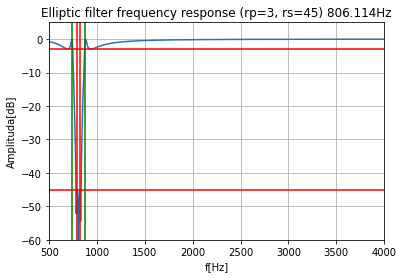
\includegraphics[scale=0.65,keepaspectratio]{Figure_10}
	\caption{Frekvenční charakteristika Elliptic filtru 1}
\end{figure}

\begin{figure}[H] 
	\centering
	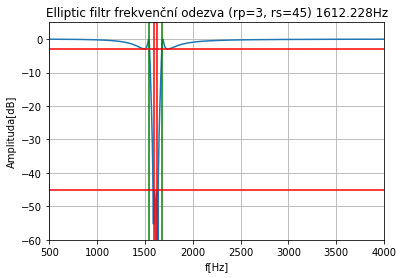
\includegraphics[scale=0.65,keepaspectratio]{Figure_11}
	\caption{Frekvenční charakteristika Elliptic filtru 2}
\end{figure}

\begin{figure}[H] 
	\centering
	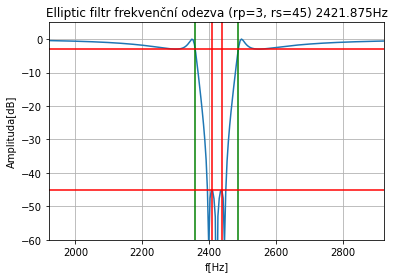
\includegraphics[scale=0.65,keepaspectratio]{Figure_12}
	\caption{Frekvenční charakteristika Elliptic filtru 3}
\end{figure}

\begin{figure}[H] 
	\centering
	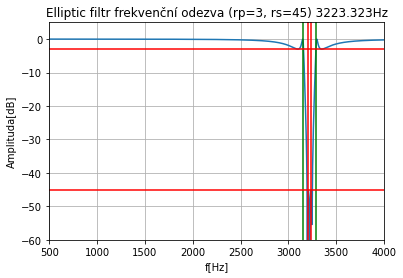
\includegraphics[scale=0.65,keepaspectratio]{Figure_13}
	\caption{Frekvenční charakteristika Elliptic filtru 4}
\end{figure}

\subsection{Butterworth filtry}
\begin{figure}[H] 
	\centering
	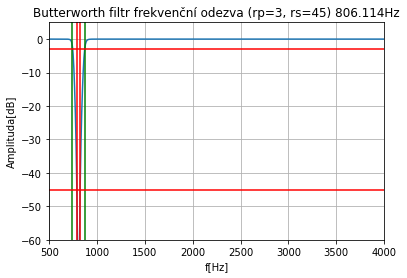
\includegraphics[scale=0.65,keepaspectratio]{Figure_14}
	\caption{Frekvenční charakteristika Butterworth filtru 1}
\end{figure}

\begin{figure}[H] 
	\centering
	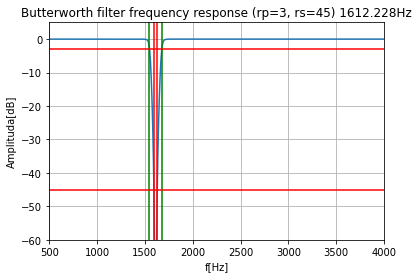
\includegraphics[scale=0.65,keepaspectratio]{Figure_15}
	\caption{Frekvenční charakteristika Butterworth filtru 2}
\end{figure}

\begin{figure}[H] 
	\centering
	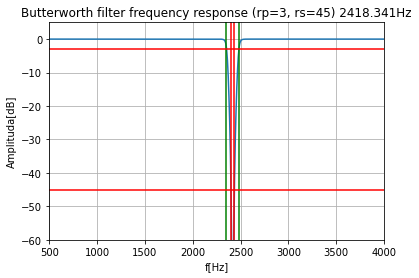
\includegraphics[scale=0.65,keepaspectratio]{Figure_16}
	\caption{Frekvenční charakteristika Butterworth filtru 3}
\end{figure}

\begin{figure}[H] 
	\centering
	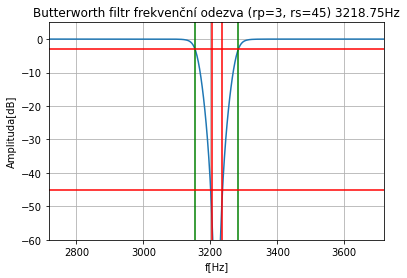
\includegraphics[scale=0.65,keepaspectratio]{Figure_17}
	\caption{Frekvenční charakteristika Butterworth filtru 4}
\end{figure}